\documentclass[letterpaper,journal]{IEEEtran}
\usepackage{amsmath,amssymb,amsfonts}
\usepackage{booktabs}
\usepackage{graphicx}
\usepackage{cite}
\usepackage{url}
\usepackage[hidelinks]{hyperref}
\usepackage{xcolor}

\newcommand{\Tr}{\operatorname{Tr}}
\newcommand{\E}{\mathbb{E}}
\newcommand{\A}{\mathcal A}
\newcommand{\T}{\mathcal T}
\newcommand{\C}{\mathbb C}
\newcommand{\SAOC}{\textsc{SAOC}}

\begin{document}

\title{Accessible Observable Contrast: Symmetry-Resolved Witnesses,
Local No-Go Certificates, and Topological Flux}

\author{Rongzhou (Lachlan) Chen%
\thanks{Working paper targeting venue fit with IEEE Transactions on Quantum
Engineering. All numerical claims are backed by fixed scripts, raw records,
tests, and manifests in the accompanying public repository. The chemistry and
robotics results are controlled models, and the gauge result is an exact
finite fixed-point benchmark, not a continuum or holographic claim.}}

\maketitle

\begin{abstract}
A discriminative observable can be physically inaccessible because it depends
on an arbitrary reference frame, violates a symmetry, or exceeds the locality
of an instrument. We formulate maximum observable contrast inside a declared
finite-dimensional observable algebra. If $\mathcal E_{\mathcal A}$ is the
trace-preserving conditional expectation onto a unital $*$-subalgebra
$\mathcal A$, the largest expectation gap over effects in $\mathcal A$ is
$\Tr[\mathcal E_{\mathcal A}(\rho_1-\rho_0)_+]$. Group twirling, fixed-region
readout, and representation-sector resolution follow as exact cases; class
states are additive and mergeable. We retain controlled validations in
translation-invariant signals, an Ising reduced state, a H{\"u}ckel difference
density, and robot contact, including ties and negative controls. We then
perform an exact 18-qubit toric-code benchmark. All 1431 Pauli observables
below code distance and all 171 one- or two-link reduced-state comparisons are
strictly blind to the selected topological-flux label. Among 22032 weight-three
Pauli strings, exactly three homologous Wilson loops have nonzero class gap.
A label-preserving logical twirl changes one-representative-per-class
inference from $0.75$ to $1$, and the learned code-space effect equals the
Wilson-sector projector; a label-flipping twirl returns chance. Helstrom
discrimination, a supplied Wilson threshold, and the learned effect all tie at
one. Thus the result establishes an observable-access hierarchy, a
symmetry-prior benefit, and a no-information certificate---not a universal
algorithmic or quantum advantage.
\end{abstract}

\begin{IEEEkeywords}
accessible observables, additive state estimation, lattice gauge theory,
quantum state discrimination, symmetry resolution, topological order,
Wilson loops
\end{IEEEkeywords}

\section{Introduction}

\IEEEPARstart{A}{n} unconstrained detector answers the wrong question when an
observer lacks an absolute phase, only a regional instrument is available, or
gauge-variant readouts are unphysical. Data augmentation may approximate an
invariance, but it does not identify the best bounded effect that is actually
available, nor certify that an entire measurement class contains no
information.

Restricted quantum measurements and invariant hypothesis testing are
established subjects~\cite{matthews2009,hiai2009}. Harmonic analysis yields
the associated representation blocks~\cite{serre1977,marvian2014}, while
symmetry-resolved entanglement decomposes reduced states by global charge
sectors~\cite{goldstein2018}. We combine these foundations with additive
positive-state summaries under the name symmetry-/subalgebra-accessible
observable contrast (\SAOC). The synthesis is deliberately broader than a
group: a fixed regional algebra and block readout are algebraic examples,
while bandwidth, bounded-weight, and other feature dictionaries define
restricted convex problems that need not be algebras.

The new question in this run is whether the same formalism can expose
topological information that every sufficiently local observer provably
misses. The toric code supplies a sharp test: orthogonal ground sectors are
locally indistinguishable, while a noncontractible Wilson loop resolves their
global flux~\cite{kitaev2003,bravyi2010}. Numerical searches for ribbon
operators~\cite{bridgeman2016} and machine learning of topological
order~\cite{che2026} already exist. We therefore do not present Wilson loops
or local topological order as discoveries.

This paper contributes:

\begin{enumerate}
\item an accessible-contrast theorem and compact-group corollary, together
with additive and mergeable class-state estimation;
\item sector diagnostics and a fixed-region no-information certificate;
\item reproducible Run 3 tests in invariant signals, many-body response,
difference-density chemistry, and robot contact with explicit strong
baselines and limitations;
\item an exhaustive $L=3$ toric-code test that moves from exact local
blindness to the first discriminative noncontractible support and checks
correct and wrong symmetry priors;
\item a quantum implementability and scaling audit that distinguishes a
compilable structured witness from a general exponentially large projector.
\end{enumerate}

\section{Accessible-Observable Theory}

\subsection{Unrestricted and algebra-restricted contrast}

Let $\rho_0,\rho_1\succeq0$ have unit trace and
$\Delta=\rho_1-\rho_0$. Over all effects $0\preceq E\preceq I$,
\begin{equation}
\max_E\Tr(E\Delta)=\Tr(\Delta_+)=\tfrac12\|\Delta\|_1,
\label{eq:helstrom}
\end{equation}
with $E^\star=\mathbf1_{\Delta>0}$. This is the Helstrom--Jordan
result~\cite{helstrom1976}, not a new quantum theorem.

Let $\A\subseteq M_d(\C)$ be a unital $*$-subalgebra and let
$\mathcal E_\A$ be its trace-preserving conditional expectation.

\textbf{Theorem 1 (accessible contrast).}
\begin{equation}
\begin{aligned}
D_\A(\rho_1,\rho_0)
&:=\sup_{\substack{E\in\A\\0\preceq E\preceq I}}\Tr(E\Delta)\\
&=\Tr[\mathcal E_\A(\Delta)_+]
=\tfrac12\|\mathcal E_\A(\Delta)\|_1 .
\end{aligned}
\label{eq:algebra}
\end{equation}
An optimizer is the positive support projector of
$\mathcal E_\A(\Delta)$, formed inside $\A$.

\begin{IEEEproof}
For $E\in\A$, Hilbert--Schmidt orthogonal projection gives
$\Tr(E\Delta)=\Tr[E\mathcal E_\A(\Delta)]$. Conditional expectation preserves
Hermiticity and maps into $\A$. The Jordan bound gives the upper bound, and
functional calculus places the positive support projector in $\A$, attaining
it.
\end{IEEEproof}

The restricted and unrestricted optima coincide exactly when an effect in
$\A$ acts as one on the positive support of $\Delta$ and as zero on its
negative support; its action on $\ker\Delta$ is arbitrary.

Equation~\eqref{eq:algebra} does not apply unchanged to an arbitrary feature
dictionary that is not closed under products and adjoints; the corresponding
restricted convex problem must then be solved directly.

\subsection{Group symmetry and sectors}

For a compact group with representation $U_g$, the commutant
$\A=\{U_g\}'$ contains invariant observables, and
\begin{equation}
\T_G(X)=\int_G U_g XU_g^\dagger\,dg
\label{eq:twirl}
\end{equation}
is the conditional expectation. Hence
\begin{equation}
\max_{\substack{0\preceq E\preceq I\\{}[E,U_g]=0}}
\Tr(E\Delta)=\Tr[\T_G(\Delta)_+].
\label{eq:symopt}
\end{equation}
If
\begin{equation}
\mathcal H=\bigoplus_\lambda V_\lambda\otimes M_\lambda,
\end{equation}
then Schur's lemma yields
\begin{equation}
\T_G(\Delta)=\bigoplus_\lambda
\frac{I_{V_\lambda}}{\dim V_\lambda}\otimes\Delta_\lambda.
\label{eq:block}
\end{equation}
Here $P_\lambda$ projects onto $V_\lambda\otimes M_\lambda$ and
$\Delta_\lambda=\Tr_{V_\lambda}(P_\lambda\Delta P_\lambda)$.
Trace norm and positive gap add over the representation sectors.

For cyclic translations, the DFT diagonalizes every invariant operator:
\begin{equation}
\T_{C_d}(|x\rangle\langle x|)
=F^\dagger\operatorname{diag}(|Fx|^2)F.
\label{eq:power}
\end{equation}
The specialized vector implementation requires $O(d\log d)$ time and $O(d)$
state per signal. The repository's general convenience path still
materializes dense matrices, so this theoretical special-case complexity is
not reported as a measured implementation advantage.

\subsection{Additive and mergeable estimation}

For encoded positive samples $\sigma(x)\succeq0$, class $c$ maintains
\begin{equation}
\begin{aligned}
S_{c,t}&=S_{c,t-1}+w_t\sigma(x_t),\\
W_{c,t}&=W_{c,t-1}+w_t,\qquad
\widehat\rho_{c,t}=S_{c,t}/W_{c,t}.
\end{aligned}
\label{eq:additive}
\end{equation}
Pairs $(S,W)$ merge by componentwise addition, so distributed sites need not
retain raw samples. A decay factor can track drift; an exact sliding window
additionally stores the samples to be deleted. General dense states cost
$O(d^2)$ memory, whereas diagonal, low-rank, stabilizer, or tensor-network
structure may reduce that cost.

\subsection{Fixed regions, local blindness, and gauge structure}

For a fixed link region $R$, the full operator algebra on $R$ is a genuine
$*$-subalgebra after extension by the identity outside $R$. Its accessible
contrast is the trace distance of the two reduced states on $R$. If $P$ is a
quantum-code projector and $R$ is correctable, the
Knill--Laflamme/local-topological-order condition is
\begin{equation}
P O_R P=c_{O_R}P
\quad\text{for every operator supported on }R.
\label{eq:localblind}
\end{equation}
It follows that all code states have the same $\rho_R$ and
$D_R=0$~\cite{knill1997,bravyi2010}. This is a no-information certificate,
not a classifier-specific failure.

Gauge theories require an additional convention: the physical Hilbert space
does not generally factor into complementary spatial tensor products, and
regional gauge-invariant algebras can have centers~\cite{donnelly2012,
casini2014}. Our ordinary link-qubit partial trace is the extended-link
(electric-center) prescription. A global-symmetry charge sector, a regional
boundary-flux sector, and a torus topological holonomy are related block
structures but are not identical.

\section{Controlled Run 3 Evidence}

Every result has raw CSV/JSON, a deterministic command, package versions,
hashes, and tests. These controlled examples test distinct consequences of
the same operator construction rather than claim universal superiority.

\subsection{Translation nuisance and quantum response}

Length-128 signals at DFT bins 5 and 17 have random cyclic shift, random
phase, Gaussian noise $0.8$, and exact sign partners. Over 12 seeds and 600
test signals per class, two training signals per class give accuracy
$0.999861$ for invariant contrast, $1.0$ for Fourier-power logistic, and
$0.5$ for both raw linear logistic and untwirled contrast. The correctly
specified Fourier baseline wins by $1.39\times10^{-4}$; the result isolates
the symmetry prior rather than a unique \SAOC\ advantage.

\begin{figure}[t]
\centering
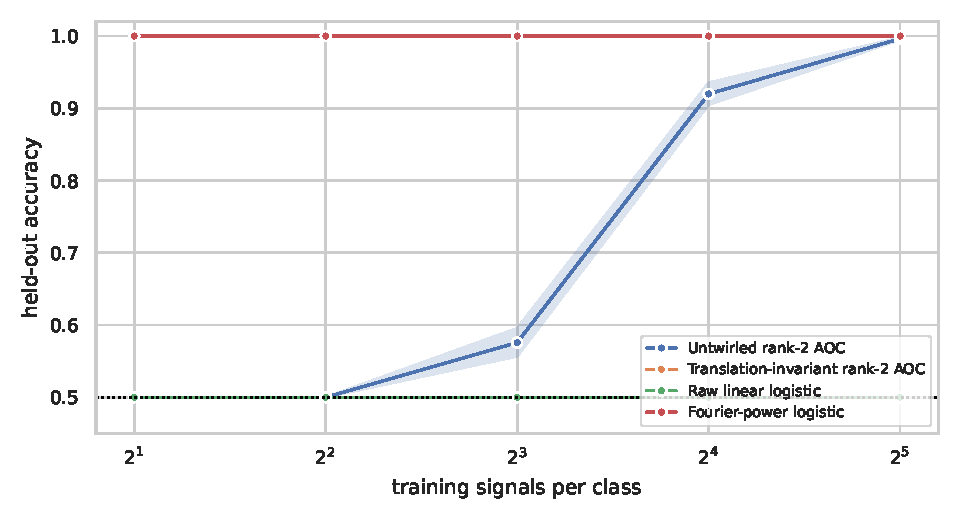
\includegraphics[width=\columnwidth]{../../experiments/run3/results/translation/translation_sample_efficiency.pdf}
\caption{Run 3 translation nuisance. Invariant contrast and the correctly
engineered Fourier baseline solve the task with one sign-pair per class; the
baseline prevents a universal-algorithm claim.}
\label{fig:translation}
\end{figure}

A ten-qubit periodic transverse-field Ising chain is exactly diagonalized,
five qubits are traced out, and adjacent reduced states are compared on a
$\delta g=0.025$ grid. The response peaks at $g/J=0.9625$, near the
thermodynamic critical value one, and the maximum parity commutator residual
is $3.54\times10^{-9}$. This is a finite-size diagnostic, not a new critical
exponent~\cite{zhang2019,khasseh2023,carrasquilla2017}.

\begin{figure}[t]
\centering
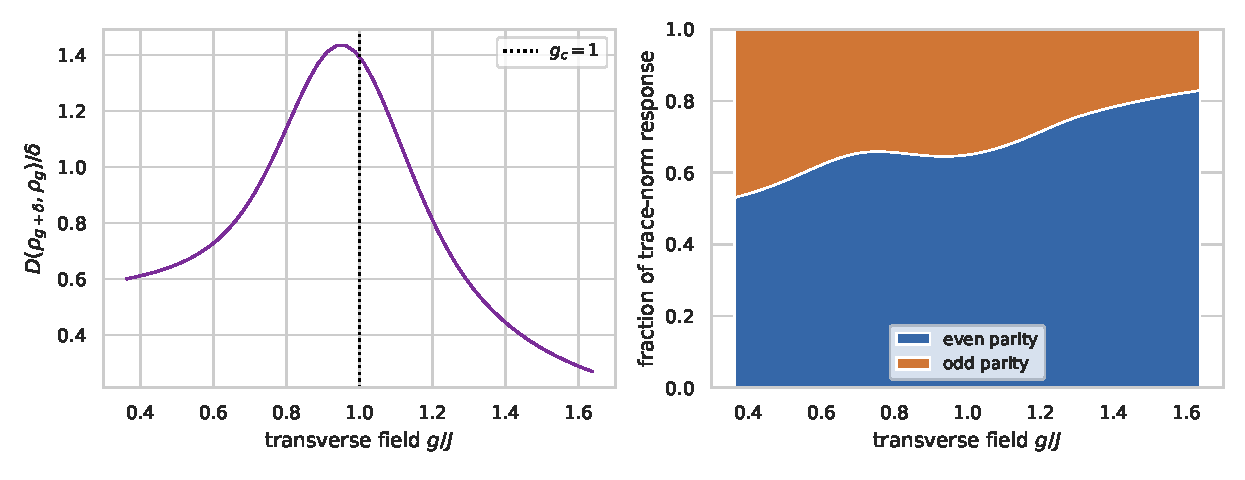
\includegraphics[width=\columnwidth]{../../experiments/run3/results/quantum_phase/symmetry_resolved_transition.pdf}
\caption{Run 3 Ising reduced-state response and parity-sector decomposition.
The dotted line is the thermodynamic critical field.}
\label{fig:quantum}
\end{figure}

\subsection{Difference-density chemistry and robot contact}

A half-filled ten-site H{\"u}ckel ring is changed from uniform to alternating
hopping. At alternation $0.7$, its one-body trace distance is $0.30845$, and
the positive and negative spectral parts define attachment and detachment
contributions whose weights balance to
$5.55\times10^{-17}$. Difference-density natural orbitals are established
chemical analysis tools~\cite{yamaki2015,bovill2026}; this is a controlled
conservation test, not quantitative molecular prediction.

A zero-mean six-axis force/torque residual receives a planted rank-one contact
covariance along a wrench screw. At 64-sample windows, the learned and oracle
scores both have ROC AUC $1.0$, mean logistic is $0.5$ by construction, and
learned/oracle screw overlap is $0.99925$. Small-window results trail the
oracle, and the experiment has neither hardware data nor an equal-budget
sample-efficiency claim.

\begin{figure}[t]
\centering
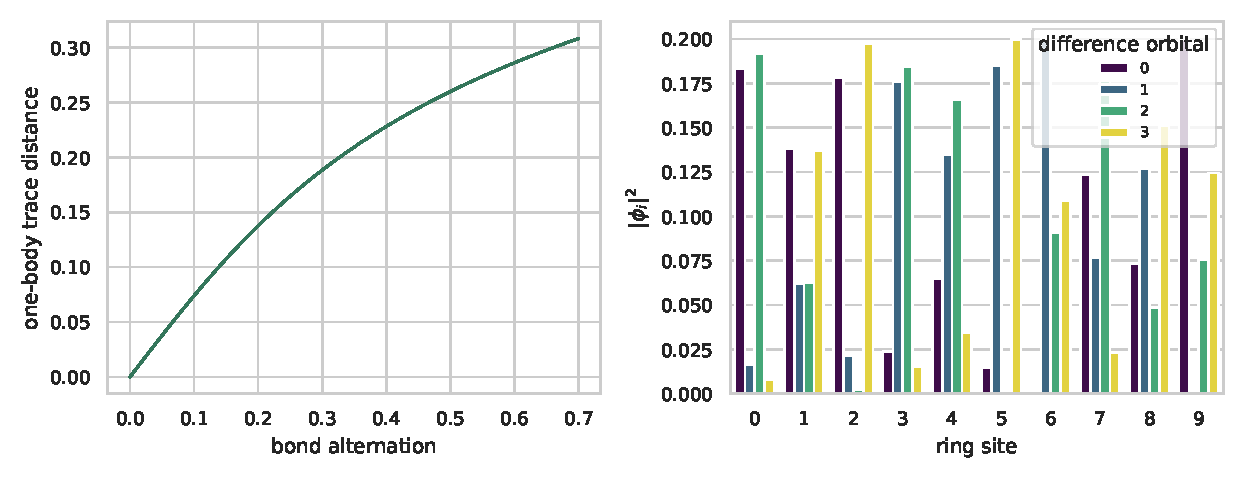
\includegraphics[width=\columnwidth]{../../experiments/run3/results/chemistry/huckel_difference_density.pdf}
\caption{Run 3 controlled H{\"u}ckel difference density and leading natural
difference orbitals.}
\label{fig:chem}
\end{figure}

\begin{figure}[t]
\centering
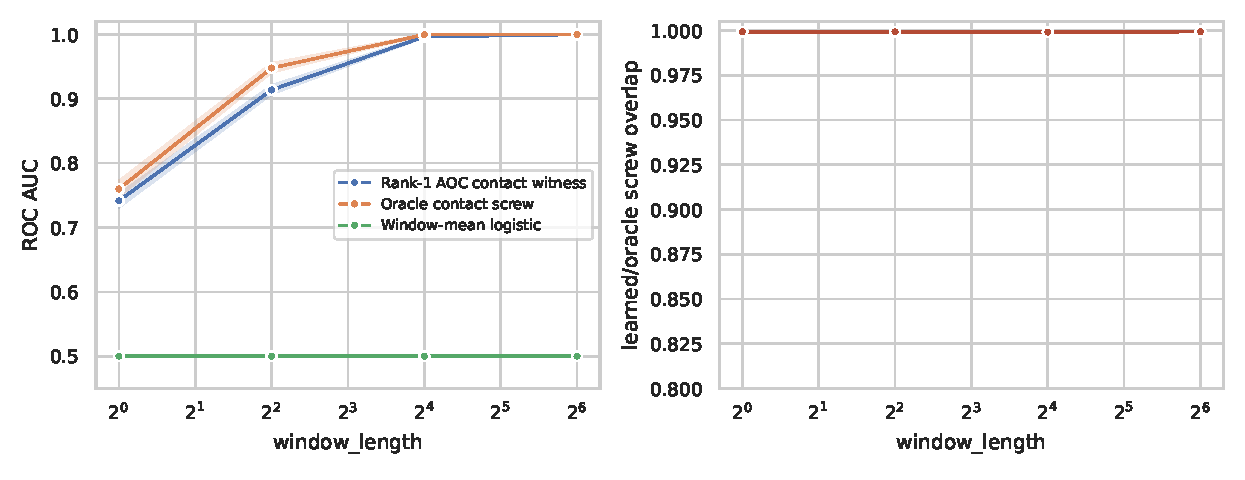
\includegraphics[width=\columnwidth]{../../experiments/run3/results/robot_contact/robot_contact_detection.pdf}
\caption{Run 3 controlled contact result. The rank-one quadratic witness
recovers the planted wrench direction; this is not deployment evidence.}
\label{fig:robot}
\end{figure}

\section{Run 4: Topological-Flux Experiment}

\subsection{Exact model and exhaustive design}

On a periodic $L\times L$ square lattice, place one qubit on each of
$2L^2$ oriented links and define
\begin{equation}
\begin{aligned}
A_s&=\prod_{e\ni s}X_e,\qquad
B_p=\prod_{e\in\partial p}Z_e,\\
H&=-\sum_s A_s-\sum_p B_p .
\end{aligned}
\label{eq:toric}
\end{equation}
For $L=3$, the 18-qubit code is $[[18,2,3]]$. We construct all four exact
ground sectors from the star group rather than diagonalize a degenerate
Hamiltonian. Every state has 256 equal-magnitude computational-basis
amplitudes and satisfies $A_s=B_p=+1$. We fix $\bar Z_y=+1$ and classify the
$\bar Z_x=\pm1$ sectors.

We exhaust all Pauli strings of weights one through three and all link subsets
of sizes one through three. No $2^{18}\times2^{18}$ density matrix is formed:
dense state vectors with 256-point sparse support and selected reduced
matrices are used. The state-vector dimension is $262144$, so this run is a
finite exact benchmark, not a scaling demonstration.

\begin{table}[t]
\centering
\caption{Exhaustive accessibility hierarchy for the selected flux label.}
\label{tab:access}
\begin{tabular}{lrr}
\toprule
Candidate class & Count & Nonzero contrast\\
\midrule
Weight-1 Pauli strings & 54 & 0\\
Weight-2 Pauli strings & 1377 & 0\\
Weight-3 Pauli strings & 22032 & 3\\
One-link RDM supports & 18 & 0\\
Two-link RDM supports & 153 & 0\\
Three-link RDM supports & 816 & 3\\
\bottomrule
\end{tabular}
\end{table}

Table~\ref{tab:access} verifies exact blindness below distance. The three
nonzero weight-three strings are the homologous horizontal $ZZZ$ Wilson loops,
with expectation gap two. Twelve weight-three Pauli strings commute with all
stabilizers, but only those three carry the selected label. For any one loop
$R$,
\begin{equation}
\rho_\pm^R=\frac{P_\pm}{2^{L-1}},\qquad
P_\pm=\frac{I\pm W}{2},\qquad
\tfrac12\|\rho_+^R-\rho_-^R\|_1=1.
\label{eq:looprdm}
\end{equation}

\subsection{Logical nuisance symmetry and controls}

In the logical basis $|a,b\rangle$, $a$ is the $\bar Z_x$ label and $b$ is an
unknown $\bar Z_y$ nuisance. Training uses one exact representative state
description $|0,0\rangle$ and $|1,0\rangle$ per class; this is not tomography
from one unknown quantum copy. Twirling over the label-preserving group
$G_{\rm nuis}=\{I,\bar X_y\}$ gives
\begin{equation}
\rho_+=\tfrac12\operatorname{diag}(1,1,0,0),\quad
\rho_-=\tfrac12\operatorname{diag}(0,0,1,1),
\label{eq:logicalstates}
\end{equation}
and, on the code space,
\begin{equation}
\Delta=\tfrac12\bar Z_x,\qquad
\operatorname{sign}(\Delta)=\bar Z_x,\qquad
E^\star=\frac{I+\bar Z_x}{2}.
\label{eq:logicaleffect}
\end{equation}
The effect outside the supported code space is not identified and is not
compared naively with a full-Hilbert-space Wilson operator.

\begin{table}[t]
\centering
\caption{Equal-prior flux-sector inference under matched test nuisance.}
\label{tab:success}
\begin{tabular}{lc}
\toprule
Method/access model & Success\\
\midrule
Any fixed $\leq2$-link observer & 0.50\\
Untwirled one-representative \SAOC & 0.75\\
No nuisance twirl (stabilized representatives) & 0.75\\
Correct nuisance twirl + \SAOC & 1.00\\
Wrong label-flipping twirl + \SAOC & 0.50\\
Supplied Wilson-parity threshold & 1.00\\
Full Helstrom oracle & 1.00\\
\bottomrule
\end{tabular}
\end{table}

The $0.75$ untwirled value uses the canonical strict-positive support and sets
the unseen kernel to zero. A kernel completion supplied with the missing
logical prior can attain one, so $0.75$ is a reproducible ablation rather than
an information-theoretic upper bound. The ``no nuisance twirl'' row is an
identity action in logical space because both representatives already satisfy
all stabilizers. The deliberately wrong group $\{I,\bar X_x\}$ flips the
label, makes the two twirled states equal, and returns chance. Correct twirling
therefore removes a nuisance; it does not manufacture information. It also
cannot increase unrestricted trace distance.

\subsection{Noise calibration}

Logical-sector mixing with probability $p$ gives
\begin{equation}
\widetilde\rho_\pm(p)=(1-p)\rho_\pm+p\rho_\mp,\quad
D(p)=|1-2p|,\quad P_{\rm succ}=1-p
\label{eq:mixing}
\end{equation}
for $0\leq p\leq1/2$. All 11 numerical points match
Eq.~\eqref{eq:mixing} exactly. With independent per-edge readout flip
probability $r$, a length-three parity is correct with
\begin{equation}
q(r)=\frac{1+(1-2r)^3}{2}.
\label{eq:readout}
\end{equation}
Majority vote over three disjoint homologous loops has success
$3q^2-2q^3$. At $r=0.05$, the values are $0.8645$ and $0.949895$,
respectively. The latter spends three times as many loop measurements and is
not an algorithm-only gain.

\begin{figure}[t]
\centering
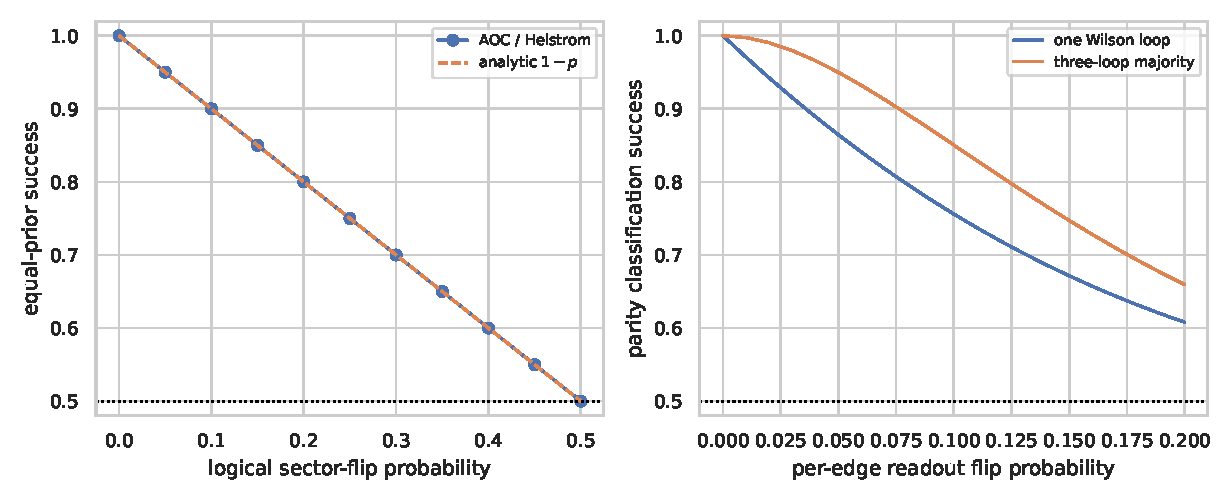
\includegraphics[width=\columnwidth]{../../experiments/run4/results/topological_flux/robustness.pdf}
\caption{Run 4 analytic calibration. Left: \SAOC\ and Helstrom coincide under
logical-sector mixing. Right: redundant homologous-loop majority improves
readout robustness at additional measurement cost.}
\label{fig:robustness}
\end{figure}

\section{Quantum Implementation and Scaling}

For the recovered structured witness, inference is a genuine quantum
measurement: measure the three-qubit Wilson parity directly, or accumulate it
on an ancilla with three controlled-NOT gates and measure the ancilla. The
projector $P_+=(I+W)/2$ is then implemented without reconstructing a global
density matrix. This is circuit compilation of a known Pauli string, not a
quantum speedup.

For a general learned dense effect, diagonalization and basis-change synthesis
are exponential in qubit count. A scalable quantum version therefore requires
additional structure: a sparse Pauli/ribbon dictionary, stabilizer or
tensor-network representation, a variational bounded observable, or a
fault-tolerant block encoding and polynomial approximation to the sign
function. The last route resembles quantum singular-value transformation but
would require efficient coherent access to class states and fault-tolerant
resources; we make no complexity advantage claim from the present simulator.

The most practical next test is not ideal-sector classification. It is
surface-code syndrome drift~\cite{dennis2002}: update additive correlation
states one round at
a time, learn a low-rank gauge-compatible change witness, and ask whether it
improves detection delay or decoder performance under equal total syndrome
rounds. Marginal-rate CUSUM, covariance detectors, decoder likelihood, known
stabilizer/Wilson diagnostics, and current correlation-aware drift methods
must be included. Universal shadow-based sequential detection~\cite{zecchin2026}
is relevant when the measurement basis is not fixed; syndrome bits are already
specific stabilizer readouts and must not be mislabeled as classical shadows.

\section{What the Results Do and Do Not Establish}

The exact Run 4 result establishes:

\begin{itemize}
\item an observable-access advantage of a noncontractible algebra over every
fixed sub-distance regional algebra;
\item a symmetry-prior advantage over untwirled one-representative learning;
\item recovery of a Wilson-equivalent code-space effect and an exact
certificate when the declared local access contains zero label information.
\end{itemize}

It does not establish superiority over Helstrom discrimination, a Wilson-loop
oracle, or logistic/threshold inference given the same parity feature. It does
not establish quantum acceleration, universal sample efficiency, scalable
tomography, a new Wilson loop or toric-code theorem, confinement, string
theory, or holographic duality. The local-indistinguishability mechanism is
known topological-order/QEC structure~\cite{kitaev2003,bravyi2010}; the
contribution is a reproducible integration of no-go certification, witness
recovery, correct/wrong symmetry controls, and noise calibration.

Likewise, the broader repository results support matched-structure
interpretation rather than universal dominance: Fourier-power logistic ties
or slightly exceeds the invariant method, optical discrimination reaches the
known Helstrom bound, and chemistry/robotics remain controlled models. A
practical advantage must be established against the strongest non-oracle
baseline using identical training, calibration, shot, and test budgets.

\section{Conclusion}

The central object is not an unconstrained feature but an effect in a declared
observable algebra. Conditional expectation projects class difference into
that algebra, its positive part gives the optimal bounded witness, sector
blocks explain where the difference resides, and additive class states admit
streaming and distributed updates. Run 3 verifies this logic across four
controlled domains. Run 4 adds a sharp topological test: the formalism first
returns an exact local no-information certificate and then recovers the
minimal Wilson-flux support when the access model permits it. The result is
mathematically exact and operationally implementable, while its advantage
remains one of representation and physical access. Circuit-level
surface-code drift under equal budgets is the next falsifiable application.

% The archived author template includes IEEEtran.cls but not IEEEtran.bst.
% Use the available numeric style for this working-paper build.
\bibliographystyle{unsrt}
\bibliography{references}

\end{document}
